\section{An toàn và bảo mật}
\label{sec:4.5}
Khi một máy tính được kết nối vào một hệ thống mạng, nó trở thành một chủ thể cho sự truy
cập bất hợp pháp và những hành động cố ý phá hoại. Trong phần này ta bàn về những
chủ đề liên quan đến vấn đề này.

\subsection*{Các dạng tấn công}

Có rất nhiều cách thức mà một hệ thống máy tính và nội dung bên trong nó có thể bị tấn
công thông qua những kết nối mạng. Rất nhiều trong số đó kết hợp với nhau chặt chẽ qua
việc sử dụng những \textbf{phần mềm độc hại} (gọi chung là malware). Những phần mềm như
vậy có thể được truyền tới, hay thực hiện trên chính máy tính chứa nó, hay nó có thể tấn
công máy tính từ một điểm cách xa. Những ví dụ của phần mềm là nó được truyền tới, và thực
hiện trên những máy tính thông qua các dạng tấn công bao gồm vi rút (virus), sâu máy tính
(worm), con ngựa thành Troa (Trojan horse), và phần mềm gián điệp (spyware), tên của chúng
phản ánh đặc tính tiêu biểu của phần mềm.

\textbf{Vi rút} là một phần mềm tiêm nhiễm vào một máy tính thông qua việc chèn thêm chính
nó vào các chương trình có sẵn trên máy tính đó. Sau đó, khi chương trình ``chủ'' được
thực thi, vi rút đó cũng được thực thi. Khi được thực thi, nhiều vi rút thực hiện một công
việc là cố gắng lây nhiễm chính bản thân chúng sang các chương trình khác trên máy
tính. Tuy nhiên, một vài vi rút thực hiện những hành động tàn phá như là làm hỏng một vài
tính năng của hệ điều hành, xóa những khối dữ liệu lớn trên bộ nhớ thứ cấp, hay làm sai
lệch dữ liệu và các chương trình khác.

\textbf{Sâu máy tính} là một chương trình tự trị mà tự động truyền nó qua một mạng máy
tính, thường trú trên các máy tính và chuyển tiếp các bản sao của chính nó sang các máy
tính khác. Cũng tương tự như trường hợp của vi rút, một sâu máy tính có thể được thiết kế
đơn thuần là tạo bản sao chính nó hay thực hiện một vài hành động phá phách mang tính nguy
hại. Một đặc tính hệ quả của sâu máy tính là sự phát triển mạnh mẽ của các bản sao sâu máy
tính làm suy biến việc thực thi của các ứng dụng hợp pháp và có thể làm cho một hệ thống
mạng hay một hệ thống liên mạng bị quá tải thực sự.

\textbf{Con ngựa thành Troa} là một phần mềm mà xâm nhập vào một hệ thống máy tính và cải
trang như là một chương trình được người dùng mong đợi, như là một trò chơi hay một gói
ứng dụng có ích, nó được nạp một cách tự nguyện bởi chính nạn nhân. Tuy nhiên, khi đã ở
trong máy tính, con ngựa thành Troa thực hiện thêm những hành động mà có thể tạo ra những
hậu quả nguy hại. Đôi khi những hành động thêm vào đó bắt đầu được thực hiện ngay lập
tức. Trong một số trường hợp, con ngựa thành Troa có thể nằm im lìm cho đến khi được kích
hoạt thông qua một sự kiện đặc biệt như sự kiện của một ngày định trước nào đó. Con ngựa
thành Troa thường đến dưới dạng là những tệp đính kèm vào những thông điệp thư điện tử hấp
dẫn, lôi cuốn người dùng. Khi tệp đính kèm được mở ra (nghĩa là khi người nhận yêu cầu xem
tệp đính kèm), những hành vi xấu xa của con ngựa thành Troa được kích hoạt. Do đó, ta
không nên mở những tệp đính kèm thư điện tử từ những nguồn không quen biết.

Một dạng khác của những phần mềm độc hại là \textbf{phần mềm gián điệp} (đôi khi còn được
gọi là \textbf{sniffing} software), là một phần mềm mà thực hiện thu thập thông tin về
những hoạt động tại máy tính mà nó thường trú và thông báo những thông tin đó về kẻ chủ
mưu của cuộc tấn công. Một vài công ty sử dụng phần mềm gián điệp như là một cách thức để
xây dựng được bộ thông tin về các khách hàng của mình, và trong trường hợp này, vẫn còn có
những nghi ngờ về phẩm chất đạo đức của họ. Trong những trường hợp khác, những phần mềm
gián điệp được sử dụng cho những mục đích hiểm độc một cách hiển nhiên như là ghi lại
những chuỗi ký tự được gõ tại bàn phím của máy tính nhằm tìm ra được mật khẩu hay số thẻ
tín dụng của người dùng.


Ngược lại với việc thu thập thông tin một cách bí mật bằng cách sniffing thông qua phần
mềm gián điệp, \textbf{phishing} là một kỹ thuật thu thập thông tin một cách rõ ràng qua
việc xin phép một cách đơn giản. Cách thức của \textit{phishing} là lợi dụng kỹ thuật moi
từ khi tiến trình liên quan được tung ra dưới dạng vô số ``tuyến'' với hy vọng một ai đó
sẽ ``bị mắc bẫy''. Phishing thường được thực hiện thông qua thư điện tử, và theo dạng này,
nó thường nhỏ gọn hơn kiểu lừa đảo cổ bằng điện thoại. Thủ phạm gửi các thông điệp thư
điện tử giả dạng dưới sự giám sát của một tổ chức tài chính, một văn phòng chính phủ, hay
có lẽ một cơ quan thi hành luật nào đó. Bức thư điện tử yêu cầu nạn nhân tiềm năng của nó
cung cấp thông tin mà được cho rằng là cần thiết cho những mục đích hợp pháp. Tuy nhiên,
thông tin thu được đó lại được sử dụng bởi chính thủ phạm phát tán thư điện tử trong những
mục đích thù địch.

Trái ngược với sự tổn thất từ những lây nhiễm cục bộ bởi vi rút và phần mềm gián điệp, một
máy tính trong một mạng có thể cũng bị tấn công bởi một phần mềm được thực hiện trên các
máy tính khác trong cùng hệ thống. Một ví dụ là \textbf{tấn công từ chối dịch vụ}, là dạng
mà một máy tính bị quá tải khi phải xử lý những yêu cầu liên tiếp. Những kiểu tấn công từ
chối dịch vụ đã bắt đầu chống lại những phần mềm phục vụ Web thương mại trên mạng Internet
nhằm đánh sập sự kinh doanh của một công ty và trong một số trường hợp có thể khiến cho
các hoạt động thương mại của công ty bị đình trệ.

Một kiểu tấn công từ chối dịch vụ đòi hỏi phát sinh một số lượng lớn các yêu cầu trong một
khoảng thời gian ngắn. Để làm được điều đó, kẻ tấn công thường gài một phần mềm trên một
số lượng lớn các máy tính không bị nghi ngờ mà từ các máy tính này sẽ phát sinh các yêu
cầu khi nhận được một tín hiệu điều khiển. Sau đó, khi tín hiệu điều khiển được đưa ra,
tất cả các máy tính này sẽ làm máy phục vụ đích bị ngập lụt bởi các thông điệp.

Như vậy, tính vốn có trong các kiểu tấn công từ chối dịch vụ chính là tính sẵn sàng sử
dụng của những máy tính không bị nghi ngờ được sử dụng như là những kẻ tòng phạm. Điều này
cũng giải thích vì sao tất cả những người sử dụng máy tính cá nhân (PC users: Personal
Computer users) được khuyến cáo là nên ngắt kết nối máy tính của mình tới mạng Internet
khi không sử dụng đến. Người ta đã ước lượng là từ khi một PC được kết nối tới mạng
Internet, ít nhất một kẻ xâm phạm nào đó sẽ cố gắng khai thác sự tồn tại của nó trong vòng
20 phút. Tóm lại, một PC không được bảo vệ có thể là mối đe dọa đáng kể tới tính toàn vẹn
của mạng Internet.

Một vấn đề khác liên quan đến một số lượng lớn các thông điệp không mong đợi là sự gia
tăng nhanh của thư rác, được gọi là \textbf{spam}. Tự nhiên, không giống như kiểu tấn công
từ chối dịch vụ, một khối lượng lớn spam ít có khả năng làm ngập lụt một hệ thống máy
tính. Thay vào đó, hậu quả của spam là khiến cho chính người nhận được spam bị ngập lụt
trong đống thư rác. Vấn đề này có thể sẽ trở nên tồi tệ hơn bởi trên thực tế, như ta
đã được giới thiệu, spam là môi trường được thông qua một cách rộng rãi giúp cho phishing
và những con ngựa thành Troa có thể làm cho máy tính bị lây nhiễm bởi vi rút và những
chương trình có hại khác.

\subsection*{Phòng chống và chữa trị}

Câu châm ngôn cổ ``Phòng bệnh còn hơn chữa bệnh'' là hoàn toàn đúng trong bối cảnh của sự
kiểm soát bởi hành động cố ý phá hoại qua những kết nối mạng. Một kỹ thuật ngăn chặn chính
là lọc giao thông truyền qua một điểm nút trên mạng, thường thông qua một chương trình gọi
là \textbf{bức tường lửa} (firewall). Ví dụ, một bức tường lửa có thể được cài đặt tại
cổng vào/ra (gateway) của một vùng nhằm lọc các thông điệp truyền vào hay ra khỏi vùng
đó. Những bức tường lửa như vậy có thể được thiết kế nhằm chặn những thông điệp đi ra với
những địa chỉ đích được chỉ định hay nhằm chặn những thông điệp đi vào từ những đích được
biết đến như là những nguồn có vấn đề. Chức năng sau này trở thành một công cụ giúp cho
việc chấm dứt một cuộc tấn công từ chối dịch vụ từ khi nó cung cấp một cách thức chặn
luồng giao thông từ những máy tính tấn công. Một vai trò phổ biến khác của bức tường lửa
tại cổng vào/ra của vùng là chặn tất cả các thông điệp đi vào mà trong đó có những địa chỉ
nguồn thuộc mạng của vùng từ đó một thông điệp như vậy sẽ chỉ ra rằng một máy trạm ngoài
vùng đang giả mạo là một thành viên trong vùng. Việc giả mạo như là một đối tác khác chứ
không phải là chính mình được biết đến với tên gọi là \textbf{spoofing}.


Những bức tường lửa cũng được sử dụng để bảo vệ các máy tính cá nhân hơn là toàn bộ hệ
thống mạng hay vùng. Ví dụ, nếu một máy tính hiện đang được dùng như là một máy chủ phục
vụ Web, một máy chủ tên miền, hay một máy chủ thư điện tử, khi đó một bức tường lửa nên
được cài đặt trên máy tính đó nhằm ngăn chặn tất cả các lưu lượng đi vào đã gửi tới các
ứng dụng đó. Thực vậy, có một cách thức mà kẻ xâm nhập bất hợp pháp có thể đoạt được toàn
quyền điều khiển một máy tính là thông qua việc thiết lập một kênh liên hệ qua một “lỗ
thủng” trên một máy chủ không hiện hữu. Đặc biệt, một phương pháp thu thập thông tin được tập
hợp bởi phần mềm gián điệp là thiết lập một phần mềm chủ bí mật trên chính máy tính đã bị
lây nhiễm bởi các ứng dụng khách nguy hại có thể truy lục được những phát hiện của phần
mềm gián điệp. Một bức tường lửa được cài đặt đúng cách có thể chặn được những thông điệp
từ những phần mềm khách nguy hại.

Một vài biến thể của các bức tường lửa được thiết kế cho những mục đích đặc biệt--một ví
dụ là các \textbf{bộ lọc thư rác}, đó là những bức tường lửa được thiết kế nhằm chặn những
thư điện tử không mong đợi. Rất nhiều bộ lọc thư rác sử dụng những kỹ thuật tinh vi, phức
tạp hơn nhằm phân biệt được đâu là thư điện tử được mong đợi và đâu là thư rác. Một vài
trong số đó học cách tạo ra sự khác biệt này qua một quá trình rèn luyện mà trong đó người
sử dụng nhận dạng được các mục chọn của thư rác cho đến khi bộ lọc thu được đủ các mẫu
nhằm đưa ra được quyết định dựa trên chính nó. Những bộ lọc này là những ví dụ về sự đa
dạng các phạm vi chủ đề (lý thuyết xác suất, trí tuệ nhân tạo,…) có thể góp phần cùng nhau
phát triển trên những lĩnh vực khác như thế nào.

Một công cụ phòng ngừa khác mà có chức năng lọc là phần mềm \textbf{máy chủ ủy nhiệm}
(proxy server). Phần mềm máy chủ ủy nhiệm là một đơn vị phần mềm đóng vai trò trung gian
giữa một phần mềm khách và một phần mềm chủ với mục đích bảo vệ phần mềm khách khỏi những
hành động có hại của phần mềm chủ. Nếu không có phần mềm máy chủ ủy nhiệm, một máy trạm
kết nối trực tiếp với một phần mềm chủ, điều đó có nghĩa là phần mềm chủ đó có  cơ hội tiếp cận trực tiếp tới
 một số lượng nhất định phần mềm khách. Trải qua một quãng thời gian, khi nhiều
máy trạm trong cùng một vùng phải đối phó với một phần mềm chủ ở xa, phần mềm máy chủ đó
có thể thu thập được vô số những thông tin về vùng này - những thông tin này có thể được
sử dụng sau đó cho mục đích tấn công vùng. Để chống lại, trong một vùng có thể cần phải có
một máy chủ ủy nhiệm chuyên biệt cho các dịch vụ (FTP, HTTP, telnet, …). Mỗi khi một máy
trạm trong vùng cố gắng liên lạc tới một trong những máy chủ dịch vụ trên, máy trạm này
thực chất là liên lạc với máy chủ ủy nhiệm. Sau đó, máy chủ ủy nhiệm sẽ đóng vai trò của
máy trạm, liên lạc với máy chủ dịch vụ ở bên ngoài. Từ đó, máy chủ ủy nhiệm đóng vai trò
trung gian giữa máy trạm thực sự và máy chủ dịch vụ ở bên ngoài vùng thông qua việc chuyển
tiếp qua lại các thông điệp. Ích lợi đầu tiên của cách bố trí này là máy chủ dịch vụ sẽ
không biết được rằng máy chủ ủy nhiệm không phải là máy trạm đang kết nối tới nó, và trên
thực tế, nó cũng không cần phải quan tâm tới sự tồn tại của máy trạm đó. Ngược lại, máy
chủ dịch vụ cũng không có cách nào mà thu thập được thông tin liên quan đến những tính
năng cục bộ của vùng. Ích lợi thứ hai là máy chủ ủy nhiệm được đặt tại vị trí mà có thể
chặn lọc tất cả các thông điệp được gửi đến máy trạm từ máy chủ dịch vụ bên ngoài vùng. Ví
dụ, một máy chủ ủy nhiệm FTP có thể kiểm tra tất cả các tệp truyền qua nó vào trong vùng
nhằm tìm ra sự hiện diện của những vi rút nhận biết được và chặn tất cả những tệp đã bị
lây nhiễm.

Vẫn còn một công cụ khác có thể ngăn chặn được những vấn đề trên trong môi trường mạng máy
tính, đó là các phần mềm kiểm định tương tự như các gói ứng dụng mà ta đã được giới thiệu
trong những thảo luận về vấn đề bảo mật hệ điều hành (Mục~\ref{sec:3.5}). Bằng việc sử
dụng các phần mềm kiểm định ở tầng mạng, người quản trị có thể phát hiện ra sự tăng thêm
đột biến trong giao thông mạng tại các vô số các vị trí khác nhau trong nội vùng, giám sát
các hoạt động của bức tường lửa trong hệ thống, và phân tích các mẫu yêu cầu được tạo ra
bởi các máy tính cá nhân riêng lẻ thuộc vùng quản lý của người quản trị nhằm phát hiện ra
những vấn đề bất hợp pháp. Trong thực tế, phần mềm kiểm định là công cụ chính của người
quản trị nhằm xác định các vấn đề trước khi nó vượt ra khỏi tầm kiểm soát.


Một cách thức khác nhằm chống lại sự xâm phạm qua các kết nối mạng là \textbf{phần mềm
  chống vi rút}, chúng được sử dụng để phát hiện và loại bỏ sự hiện diện của những vi rút
nhận biết được và sự lây nhiễm khác. (Thực tế, phần mềm chống vi rút là đại diện cho một
lớp các sản phẩm phần mềm, mỗi phần mềm đó được thiết kế nhằm phát hiện và gỡ bỏ một loại
lây nhiễm cụ thể. Ví dụ, trong khi rất nhiều sản phẩm thực sự chuyên biệt hóa trong việc
kiểm soát vi rút, những sản phẩm khác lại chuyên biệt hóa trong việc bảo vệ khỏi các phần
mềm gián điệp.) Đối với những người sử dụng các phần mềm này, có thể nói là rất quan trọng
để hiểu rằng chỉ khi trong trường hợp của những hệ thống sinh học, những sự lây nhiễm máy
tính mới là liên tục xảy ra do đó yêu cầu các phần mềm chống vi rút phải được cập nhật
thường xuyên. Ngoài ra, phần mềm chống vi rút cũng phải được bảo trì thường xuyên bằng cách tải
những bản cập nhật từ nhà cung cấp phần mềm đó. Tuy nhiên, thậm chí trong trường hợp này
cũng có thể vẫn không đảm bảo được sự an toàn cho máy tính. Sau cùng, một vi rút mới phải
lây nhiễm trước tiên vào một vài máy tính trước khi nó bị phát hiện ra và một bản cập nhật
mới được đưa ra sau đó. Chính vì vậy, một người sử dụng máy tính sáng suốt là không bao
giờ mở những tệp đính kèm thư điện tử xuất phát từ những nguồn không quen biết, không tải
những phần mềm mà không có sự tin tưởng, không trả lời các cửa sổ quảng cáo mở ra bất
chợt, và không kết nối PC vào mạng Internet khi không cần thiết.


\subsection*{Mã hoá}

Trong một số trường hợp, mục đích của những hành động phá hoại mạng máy tính là làm sập
toàn bộ hệ thống (như trong trường hợp tấn công từ chối dịch vụ), nhưng trong những trường
hợp khác thì mục đích thực sự lại là đoạt quyền truy cập tới những thông tin quý
giá. Những cách thức cổ điển của việc bảo vệ thông tin là điều khiển truy cập nó thông qua
việc sử dụng mật khẩu. Tuy nhiên, mật khẩu có thể bị dàn xếp và cũng là một giá trị
khi dữ liệu được truyền qua các mạng và liên mạng nơi mà các thông điệp được chuyển tiếp
bởi những đối tượng không nhận biết được. Trong những trường hợp như vậy, việc mã hóa có
thể được sử dụng để ngay cả nếu dữ liệu bị rơi vào tay của tin tặc, thông tin được
mã hóa sẽ vẫn duy trì được tính mật của nó. Ngày nay, rất nhiều các ứng dụng Internet cổ
điển đã biến đổi bằng cách kết hợp với các kỹ thuật mã hóa, và đưa ra những ứng dụng với
``những phiên bản an toàn'' (secure versions). Ví dụ như \textbf{FTPS}, là một phiên bản
an toàn của FTP, và SSH như ta đã được giới thiệu trong Mục~\ref{sec:4.2} là một bản thay
thế an toàn của telnet.

Vẫn còn có một ứng dụng khác là phiên bản an toàn của HTTP, được biết đến với tên gọi
\textbf{HTTPS}, mà được sử dụng bởi hầu hết các cơ quan tài chính nhằm cung cấp cho khách
hàng một cách thức truy cập an toàn tới tài khoản của họ. Cột trụ của HTTPS là hệ thống
giao thức \textbf{SSL (Secure Sockets Layer)}, mà tiền thân được phát triển bởi Netscape
nhằm cung cấp một cách thức kết nối truyền thông an toàn giữa các ứng dụng khách Web và
các ứng dụng phục vụ. Hầu hết các trình duyệt đều chỉ ra cách thức sử dụng SSL thông qua
việc hiển thị một biểu tượng cái khóa nhỏ trên màn hình máy tính. (Một vài trình duyệt sử
dụng sự hiện diện hay vắng mặt của biểu tượng này chỉ ra là SSL có được sử dụng hay không,
những trình duyệt khác lại hiển thị cái khóa ở trạng thái được khóa hay không được khóa.)

Một trong những kỹ thuật khá hấp dẫn trong lĩnh vực mã hóa là \textbf{mã hóa khóa công
  khai} (public-key), kỹ thuật này là một hệ thống mã hóa mà nó cho biết làm thế nào để mã
hóa các thông điệp sao cho không cho phép bất kỳ ai có thể giải mã được chúng--một đặc
tính mà xem như là khác thường. Xét cho cùng, khả năng trực giác sẽ gợi ra rằng một người
mà biết được các thông điệp được mã hóa như thế nào sẽ có khả năng đảo ngược lại quá trình
nhằm giải mã được các thông điệp đó. Nhưng điều này là không thể xảy ra khi kỹ thuật mã
hóa khóa công khai được sử dụng.



Một hệ thống mã hóa khóa công khai đòi hỏi phải sử dụng hai giá trị được gọi là khóa. Một
khóa, được biết đến với tên gọi là \textbf{khóa công khai}, được sử dụng để mã hóa các
thông điệp; khóa còn lại, với tên gọi là \textbf{khóa bí mật}, được sử dụng để giải mã các
thông điệp. Để sử dụng hệ thống này, khóa công khai trước tiên cần phải được phân phát tới
cho những ai cần để gửi những thông điệp tới một đích nào đó. Khóa bí mật được giữ lại một
cách tin cậy tại đích nhận thông điệp. Sau đó, người gửi thông điệp có thể mã hóa thông
điệp bằng cách sử dụng khóa công khai và gửi thông điệp đó tới đích nhận với sự đảm bảo là
nội dung của nó được an toàn, thậm chí nếu nó bị chặn và được thu thập bởi một người trung
gian biết được khóa công khai. Thực vậy, chỉ có người nhận thông điệp đó một cách hợp pháp
và giữ khóa bí mật mới có thể giải mã được thông điệp. Do đó nếu Bob tạo ra một hệ thống
mã hóa công khai và trao cho Alice và Carol khóa công khai, sau đó cả Alice và Carol có
thể mã hóa các thông điệp rồi gửi cho Bob, nhưng họ không thể do thám được quá trình liên
lạc của người khác. Vậy là nếu Carol chặn đứng được một thông điệp được gửi từ phía Alice
cho Bob, cô ta cũng không thể giải mã được nó cho dù cô ta có biết được cách thức Alice mã
hóa nó như thế nào (Hình~\ref{fig:fig4.16}).
\begin{figure}[tbh] 
  \centering \scalebox{0.5}{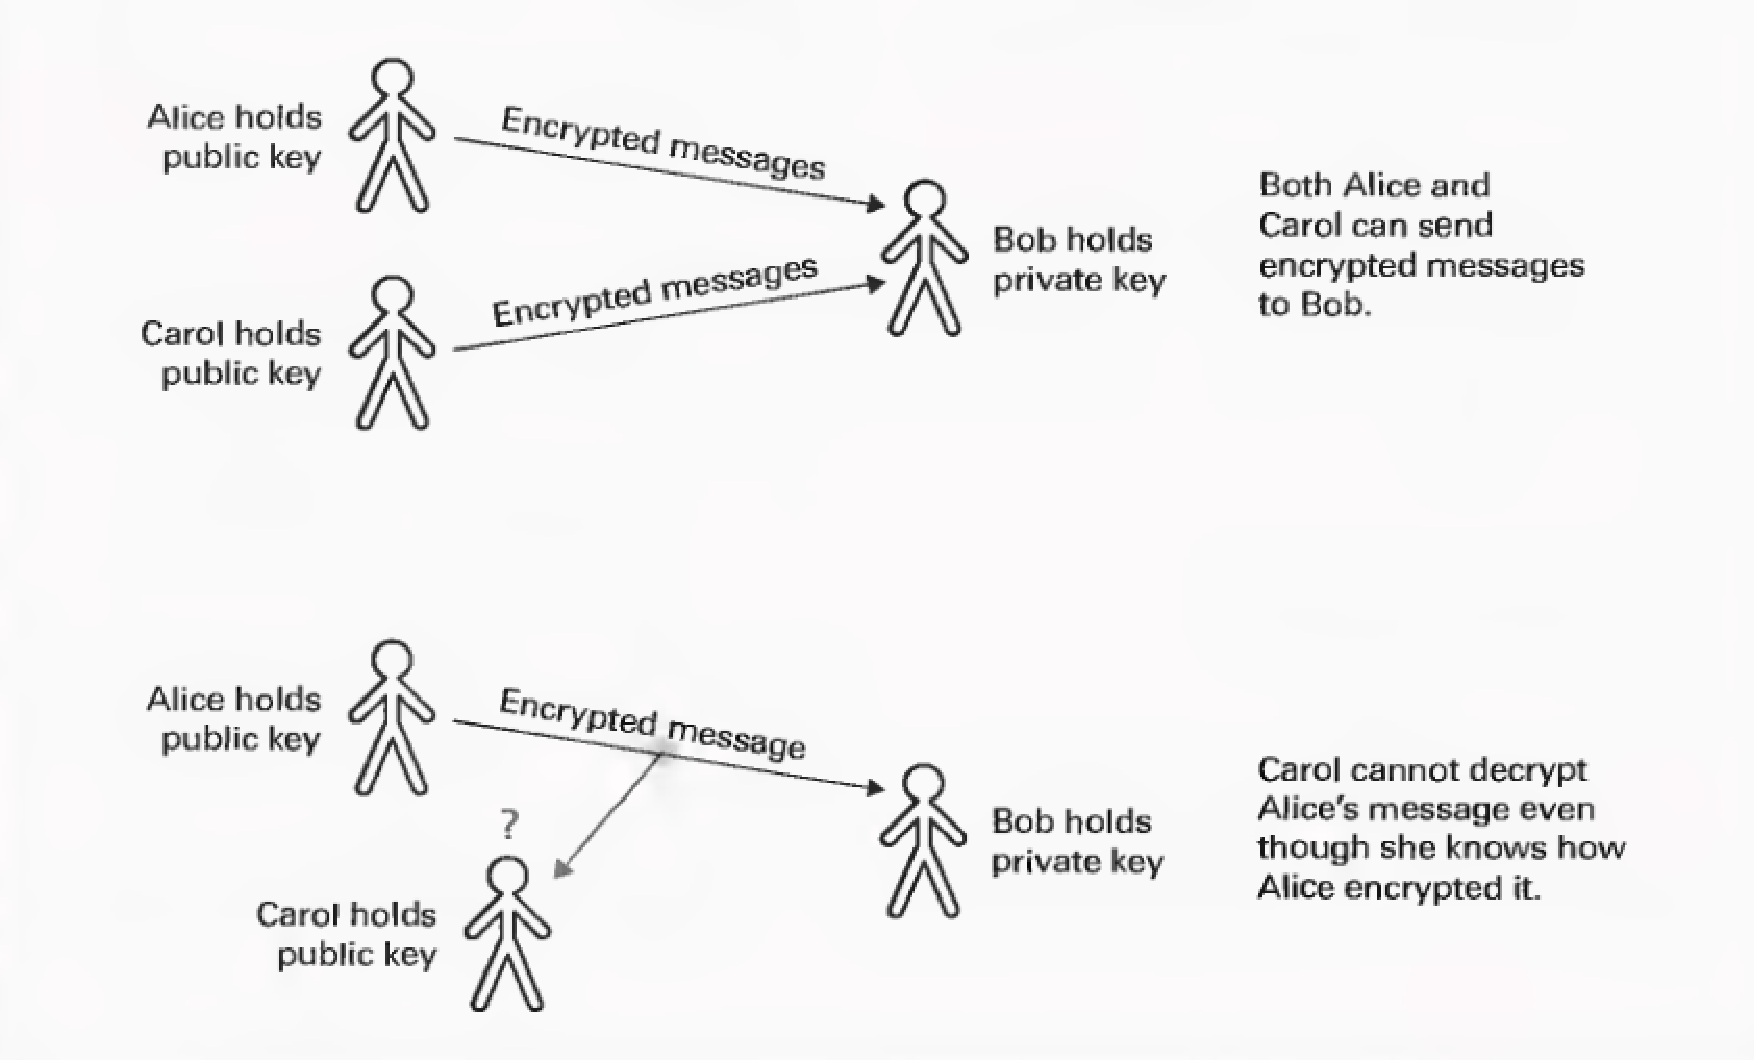
\includegraphics{ch5/fig416.pdf}}
  \caption{Mã khoá công khai}
  \label{fig:fig4.16}
\end{figure}

Tất nhiên, vẫn có những vấn đề không dễ phát hiện bị che dấu trong hệ thống mã hóa khóa
công khai. Một là phải đảm bảo rằng khóa công khai đang được sử dụng là khóa hợp pháp cho
người nhận thông điệp. Ví dụ, nếu bạn đang giao dịch với ngân hàng của bạn, bạn muốn chắc
chắn rằng khóa công khai mà bạn đang sử dụng để mã hóa là đúng của ngân hàng và nó không
bị mạo danh. Nếu một kẻ mạo danh tự giới thiệu là ngân hàng (một quá trình đã được giới
thiệu trước đó là spoofing) và đưa cho bạn khóa công khai của nó, các thông điệp mà bạn mã
hóa và gửi tới ``ngân hàng'' sẽ là có ý nghĩa đối với kẻ mạo danh chứ không phải cho ngân
hàng của bạn. Do đó, nhiệm vụ kết hợp các khóa công khai với các tổ chức uy tín là rất cần
thiết.

Một cách tiếp cận để có thể giải quyết được vấn đề này là thiết lập các điểm tin cậy trên
mạng Internet, thường được gọi là các \textbf{tổ chức chứng thực số} (CA: Certificate
Authority), nhiệm vụ của những tổ chức này là duy trì danh sách các đối tác cùng với các
khóa công khai của họ. Những tổ chức này, hoạt động dưới hình thức là các ứng dụng chủ,
sau đó cung cấp thông tin về khóa công khai tin cậy tới các ứng dụng khách thông qua các
gói được biết đến như là các chứng chỉ (certificates). Một \textbf{chứng chỉ số} là một
gói bao gồm tên của người tham gia và khóa công khai của anh ta hay cô ta. Ngày nay có rất
nhiều các tổ chức chứng thực số thương mại tồn tại trên mạng Internet, mặc dù nó cũng phổ
biến đối với các tổ chức nhằm duy trì chứng thực số của chính bản thân họ để bảo vệ sát sao việc điều khiển những hệ thống truyền thông vượt tầm kiểm soát của họ.

Cuối cùng, ta cũng nên bình luận về vai trò của những hệ thống mã hóa khóa công khai
trong việc giải quyết các vấn đề liên quan đến quá trình tạo sự \textbf{thẩm định quyền
  hạn} mà trên thực tế tác giả của một thông điệp cần gửi đi chính là người tham gia. Điểm
mấu chốt cần phê bình ở đây là trong những hệ thống mã hóa khóa công khai, vai trò của
khóa mã hóa và khóa giải mã có thể hoán đổi cho nhau. Thật vậy, văn bản có thể được mã hóa
bằng khóa bí mật, và khi chỉ có người tham gia vào hệ thống mới có quyền truy cập vào khóa
đó, bất kỳ văn bản nào được mã hóa đều phải bắt nguồn từ người tham gia đó. Theo cách này,
người giữ khóa bí mật có thể đưa ra một mẫu bít, gọi là chữ ký số, mà chỉ có người tham
gia hệ thống mới biết được cách thức sinh ra chữ ký số đó như thế nào. Bằng cách đính kèm
chữ ký số đó vào thông điệp, người gửi có thể chứng tỏ thông điệp cần gửi là đáng tin
cậy. Một chữ ký số có thể đơn giản như phiên bản mã hóa của chính thông điệp. Tất cả công
việc mà người gửi phải thực hiện là mã hóa thông điệp sẽ được truyền bằng cách sử dụng
khóa bí mật của anh ta hay cô ta (khóa mà được sử dụng để giải mã). Khi thông điệp được
nhận, người nhận sẽ dùng khóa công khai của người gửi để giải mã chữ ký số trong thông
điệp. Thông điệp đó đã thể hiện rõ là được đảm bảo đáng tin cậy bởi vì chỉ có người giữ khóa bí
mật mới có thể đưa ra được phiên bản mã hóa.

\subsection*{Những cách thức tiếp cận hợp pháp tới vấn đề an ninh mạng}
Một cách thức cho phép gia tăng sự an toàn của những hệ thống mạng máy tính là áp dụng các
biện pháp phòng chống mang tính pháp lý. Tuy nhiên, cũng có hai vấn đề trở ngại đối với
cách tiếp cận này. Trước tiên đó là việc tạo ra một hành động bất hợp pháp không ngăn chặn
được hành động đó. Tất cả những việc mà nó thực hiện là cung cấp một sự giúp đỡ hợp
pháp. Vấn đề trở ngại thứ hai là trạng thái nguyên thủy của các phương tiện hoạt động mạng
quốc tế thường rất khó khăn để có được sự giúp đỡ. Điều gì là bất hợp pháp đối với một
quốc gia có thể lại là hợp pháp đối với quốc gia khác. Cuối cùng thì việc gia tăng mức độ
an toàn của hệ thống mạng bằng các phương tiện pháp lý là một dự án quốc tế, và do đó cần
phải được thực hiện bởi những hội đồng hợp pháp--mà tổ chức có tiềm năng nhất là Tòa án
quốc tế (International Court of Justice) tại Hague.

Sau khi đã đưa ra những lời phủ nhận, ta cũng phải thừa nhận rằng, mặc dù chưa hoàn
hảo hơn, các lực lượng pháp lý cũng có một sự ảnh hưởng rất lớn, và do đó ta phải có
nhiệm vụ khám phá ra các bước hợp pháp mà đã đang được sử dụng để giải quyết các vấn đề
xung đột trong các hoạt động liên quan đến mạng máy tính. Với mục đích này, ta sử
dụng các ví dụ lấy ra từ các luật lệ liên bang của Hoa Kỳ. Những ví dụ tương tự có thể
được rút ra từ các cơ quan chính phủ của Liên minh Châu Âu.

Ta bắt đầu với sự gia tăng của phần mềm độc hại. Tại Hoa Kỳ, vấn đề này được chỉ ra
bởi luật Gian lận trong máy tính và Lạm dụng đạo luật (Computer Fraud and Abuse Act), mà
lần đầu tiên được thông qua năm 1984, mặc dù nó đã được sửa đổi nhiều lần. Đó là hành động
dưới này mà hầu hết các trường hợp liên quan đến việc giới thiệu về sâu và vi rút đã bị
truy tố. Tóm lại, các đạo luật đòi hỏi phải chứng minh rằng các bị đơn cố tình truyền tải
một chương trình hay dữ liệu có thể gây ra thiệt hại.


Đạo luật Gian lận trong máy tính và Lạm dụng đạo luật cũng bao gồm các trường hợp liên
quan đến sự hình thành hành vi trộm cắp. Đặc biệt, các hành động phạm pháp sẽ nhận được
bất cứ điều gì về giá trị thông qua việc truy cập trái phép vào một máy tính. Các phiên
toà có xu hướng chỉ định một mở rộng để làm sáng tổ cụm từ ``bất cứ điều gì về giá trị,''
và như vậy, đạo luật Gian lận trong máy tính và Lạm dụng Đạo luật đã được áp dụng nhiều
hơn cho các hành vi trộm cắp thông tin. Ví dụ, tòa án có quy định rằng các chỉ sử dụng một
máy tính có thể cấu thành nên ``bất cứ điều gì về giá trị.''

Sự đúng đắn của vấn đề riêng tư là ở chỗ khác, và có lẽ hầu hết đều gây ra các cuộc tranh
luận, các hoạt động mạng thường đối mặt với các vấn đề cơ sở pháp lý trong cộng đồng. Các
câu hỏi liên quan đến quyền giám sát những thông tin liên lạc từ phía các nhân viên của
một ông chủ và sự phản ảnh mức độ một nhà cung cấp dịch vụ Internet có thẩm quyền để truy
cập thông tin được truyền đạt bởi các khách hàng của nó đã tạo ra được số lượng đáng kể
những ý tưởng. Ở Hoa Kỳ, rất nhiều câu hỏi đã được đưa ra bởi Electronic Communication
Privacy Act (ECPA) vào năm 1986, có nguồn gốc của nó trong luật pháp để kiểm soát
wiretapping. Mặc dù các hành động kéo dài một cách nhàm chán, nhưng mục đích của nó có
được một vài trích dẫn ngắn ngủi. Đặc biệt, nó cũng nói rõ rằng

\begin{quotation} \small Trừ khi có những quy định cụ thể khác đã được đưa ra trong chương
  này, bất kỳ ai có ý chặn, cố gắng chặn, hay dẫn dắt người nào đó chặn hay cố gắng chặn
  bất kỳ một đoạn thư tín, một cuộc nói chuyện, hay một giao dịch điện tử… đều sẽ bị phạt
  theo quy định đã đề ra trong phần (4) hay sẽ bị giám sát nhu cầu theo quy định đề ra
  trong phần (5).
\end{quotation}
và
\begin{quotation} \small …bất kỳ cá nhân hay một tổ chức cung cấp dịch vụ truyền thông
  điện tử cho công chúng sẽ không được tiết lộ nội dung của bất kỳ một giao dịch truyền
  thông nào… mà dịch vụ đó được gửi tới bất kỳ ai hay một tổ chức nào đó chứ không chỉ đơn
  thuần là một cá nhân nhận thư hay nhận một giao dịch truyền thông như vậy hay một nhóm
  người nhận.
\end{quotation}


Tóm lại, ECPA xác định quyền giao tiếp của một cá nhân, đó là bất hợp pháp đối với một nhà
cung cấp dịch vụ Internet để phát hành các thông tin về sự truyền thông của các khách
hàng, và nó là bất hợp pháp cho nhân viên không có thẩm quyền nghe lén trái phép một cuộc
giao tiếp của người khác. Nhưng ECPA lại rời bỏ khỏi cuộc tranh luận. Ví dụ, các câu hỏi
liên quan đến các quyền của một chủ nhân để giám sát các giao tiếp của nhân viên sẽ trở
thành một vấn đề liên quan đến sự cấp phép, mà các toà án có xu hướng cấp quyền cho người
sử dụng lao động khi sự truyền thông được thực hiện bằng cách sử dụng các thiết bị của họ.


Hơn nữa, các hoạt động được tiếp tục trình lên một số cơ quan chính phủ có thẩm quyền để
giám sát sự truyền thông điện tử với một số hạn chế nhất định. Các điều khoản này đã trở
thành nguồn gốc của nhiều tranh cãi. Ví dụ, trong năm 2000, FBI tiết lộ sự tồn tại của hệ
thống, gọi là Carnivore, tiết lộ đó chỉ đưa ra các báo cáo về sự truyền thông của tất cả
các thuê bao thuộc một nhà cung cấp dịch vụ Internet hơn là một tòa án thiết kế nhắm mục
tiêu, và vào năm 2001 để phản ứng lại sự tấn công khủng bố trên Trung tâm Thương mại Thế
giới, hội Mỹ thông qua vấn đề USA PATRIOT (Liên minh Tăng cường Mỹ do cung cấp các Thích
hợp Công cụ bắt buộc để ngăn cản trở và khủng bố) Luật sửa đổi các hạn chế mà theo đó các
cơ quan chính phủ phải hoạt động.

\begin{figure}
  \begin{quotation}
    \noindent
    \textbf{Các đội phản ứng khẩn cấp máy tính}\vspace{0.3cm}
    \\
    Trong tháng 11 năm 1988, một sâu máy tính đã được thả vào Internet và đã gây ra sự sụp
    đổ một cách đáng kể các dịch vụ. Do đó, Cơ quan nghiên cứu các dự án cao cấp của Hoa
    Kỳ đã hình thành Đội phản ứng khẩn cấp máy tính CERT (CERT được đánh vần là ``SERT''),
    được đặt tại Trung tâm điều phối CERT tại trường Đại học Carnegie-Mellon. CERT chính
    là trung tâm quản lý sự an toàn của Internet (``watchdog''). Một trong số nhiệm vụ của
    trung tâm này là điều tra về các vấn đề an ninh, đưa ra các cảnh báo về an ninh, và
    thực hiện các chiến dịch nhận thức công cộng để cải thiện an ninh Internet. Trung tâm
    CERT duy trì một trang web có địa chỉ là \url{http://www.cert.org} mà tại đó đăng tải
    các bài viết, những thông báo về các hoạt động của nó.
  \end{quotation}
\end{figure}

%%% Local Variables: 
%%% mode: latex
%%% TeX-master: "../tindaicuong"
%%% End: 
